% introduction.tex

\section{Introduction}
\label{sec:introduction}
Traffic congestion is a growing problem that continues to plague urban areas with negative outcomes to both the traveling public and society as a whole. These negative outcomes will only grow over time as more people flock to urban areas. In 2014, traffic congestion costs Americans over \$160 billion in lost productivity and wasted over 3.1 billion gallons of fuel~\cite{Econ14}. Traffic congestion was also attributed to over 56 billion pounds of harmful CO2 emissions in 2011~\cite{schrank20152015}. 
In the European Union, the cost of traffic congestion was equivalent to 1\% of the entire GDP~\cite{schrank2012tti}.
Mitigating congestion would have significant economic, environmental and societal benefits.
Signalized intersections are one of the most prevalent bottleneck types in urban environments, and thus traffic signal control plays a vital role in urban traffic management.

\begin{figure}[htbp]
\centering
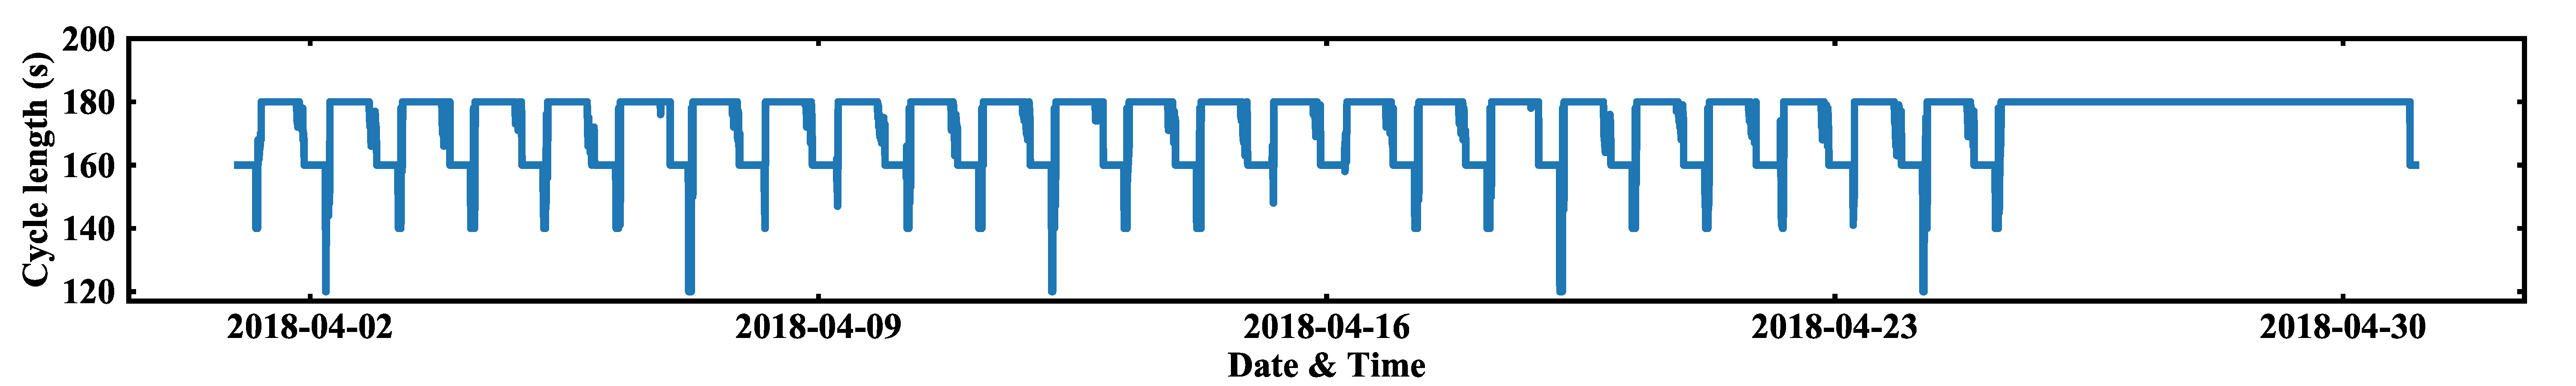
\includegraphics[width=0.99\textwidth]{figures/timing.pdf} 
\caption{Traffic signal timing in a city. The cycle length rarely changes.}
\label{fig:timing}
\end{figure}


\subsection{Current Situation}
In many modern cities today, the widely-used adaptive traffic signal control systems such as SCATS~\cite{SCATS} and SCOOT~\cite{hunt1981scoot,hunt1982scoot} heavily rely on manually designed traffic signal plans. Such manually set traffic signal plans are designed to be dynamically selected according to the traffic volume detected by loop sensors. However, many intersections do not have loop sensors installed or the loop sensors are poorly maintained. Moreover, the loop sensors are activated only when vehicles pass through them, thus they can only provide partial information about the vehicle through them. As a result, the signal cannot perceive and react to the real-time traffic patterns, and engineers need to manually change the traffic signal timings in the signal control system under certain traffic condition scenarios. Figure~\ref{fig:timing} shows the traffic signal timing at an intersection in a city of China and the traffic signal timing rarely changes regardless of the real traffic changes throughout the day.


\subsection{Opportunities}
\emph{First, today we have much richer information that can be collected from various sources.} Traditional traffic signal control relies on data from loop sensors, which can only sense the vehicle passing. However, new data sources are quickly becoming available that can serve as input for traffic signal control purposes. For instance, street-facing surveillance cameras used for security purposes can also provide a more detailed depiction of  the traffic situation on nearby roads -- specifically, how many cars are waiting in the lane, how many cars are taking turns, where they are located, and how fast they are traveling. In addition, large-scale trajectory data can be collected from various sources such as navigation applications (e.g., Google Maps),  ride-sharing platforms (e.g., Uber) and GPS-equipped vehicles that share information with the nearby infrastructure (e.g., connected vehicles). Such data provide us with more insight about how vehicles arrive to intersections. We have reached a stage of abundant mobility information that can describe the traffic dynamics in the city more clearly, which is an essential resource for us to improve the traffic control system.


 
\begin{figure}[htbp]
\centering
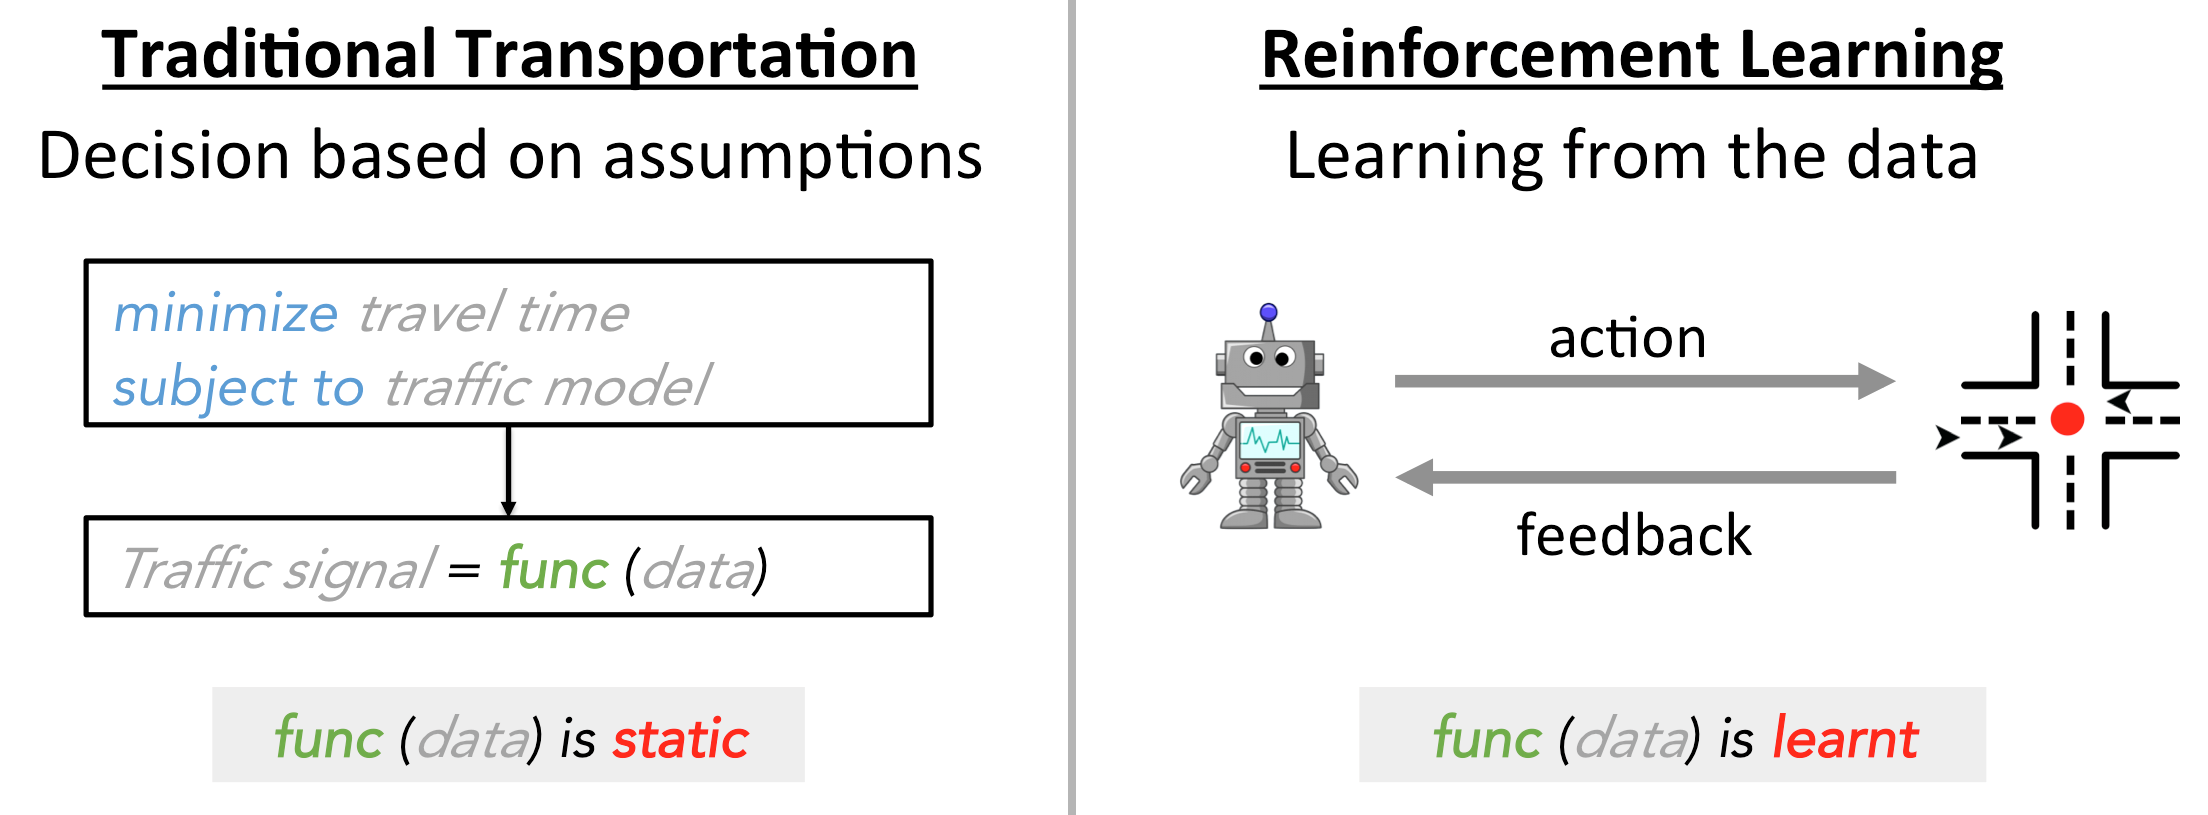
\includegraphics[width=0.7\columnwidth]{figures/optimizationvsRL.png}
\caption{Difference between traditional transportation approach and machine learning approach.}
\label{fig:optvsrl}
\end{figure}

\emph{Second, today we have much stronger computing power and advanced computational models.} The typical approach that transportation researchers take is to cast traffic signal control as an optimization problem under certain assumptions about the traffic model, e.g., vehicles come in a uniform and constant rate~\cite{RPM04}.  Various (and sometimes strong) assumptions have to be made in order to make the optimization problem tractable. The key issue here is that these assumptions deviate from the real world and often do so significantly. As we know, real-world traffic condition evolves in a complicated way, affected by many factors such as driver's preference, interactions with vulnerable road users (e.g. pedestrians, cyclists, etc.), weather and road conditions, just to name a few. These factors can hardly be fully described in a traffic model.


On the other hand, machine learning techniques can directly learn from the observed data without making unrealistic assumptions about the model. However, typical supervised learning does not apply here because existing traffic signal control systems follow pre-defined signal plans so we do not have enough training data to differentiate good and bad traffic signal plan strategies. Instead, we have to first take actions to change the signal plans and then learn from the outcomes. This trial-and-error approach is also the core idea of reinforcement learning (RL). In essence, an RL system generates and executes different strategies (e.g., for traffic signal control) based on the current environment. It will then learn and adjust the strategies based on the feedback from the environment. This reveals the biggest difference between transportation approaches and our RL approaches, which is illustrated in Figure~\ref{fig:optvsrl}: in traditional transportation research, the model $func(data)$ is static; in reinforcement learning, the model is dynamically learned through trial-and-error in the real environment.




